\chapter{Cables}\index{cables}

Es tracten en aquest cap\'{\i}tol q\"{u}estions relatives als cables el\`{e}ctrics.

\section{Resist\`{e}ncia}\index{cables!resist\`{e}ncia}

\subsection{Resist\`{e}ncia d'un conductor}

La resist\`{e}ncia $R$ d'un conductor dep\`{e}n de la resistivitat $\rho$
del material, de la llargada $l$ del conductor i de la seva secci\'{o}
$S$.
\begin{equation}
   R= \rho \frac{l}{S}
\end{equation}
\index{$\rho$}

\index{resistivitat!variaci\'{o} amb la temperatura}La resistivitat no
\'{e}s un valor constant, sin\'{o} que dep\`{e}n de la temperatura; a major
temperatura, major resistivitat. Coneixent la resistivitat $\rho_1$ a una
temperatura $T_1$, es pot calcular la resistivitat $\rho_2$ a una altra
temperatura $T_2$, a partir del coeficient de variaci\'{o} de la
resistivitat amb la temperatura $\alpha_1$, donat a la temperatura $T_1$.
\begin{equation}
   \rho_2 = \rho_1 [1 + \alpha_1 (T_2 - T_1)]\label{eq:resistivitat}
\end{equation}
\index{$\alpha$}

\index{resistivitat!valors}En la Taula
\vref{taula:param-elc} es donen valors de la resistivitat i dels
coeficients de variaci\'{o} de la resistivitat amb la temperatura, a
20\unit{\celsius} i a 0\unit{\celsius}, per a diversos materials.
\begin{table}[htb]
   \caption{\label{taula:param-elc} Par\`{a}metres el\`{e}ctrics d'alguns materials}
   \[ \begin{array}{lccc}
   \toprule[1pt]
   \text{Material} & \rho_{20\unit{\celsius}}\unit{[\ohm\,mm^2/m]} & \alpha_{20\unit{\celsius}}\unit{[\celsius^{-1}]} &
   \alpha_{0\unit{\celsius}}\unit{[\celsius^{-1}]}
   \\
   \midrule
      \text{Alumini} & 0{,}02825 & 0{,}00391 & 0{,}00424 \\
      \text{Coure}   & 0{,}01723 & 0{,}00393 & 0{,}00427 \\
      \text{Plata}   & 0{,}01645 & 0{,}00380 & 0{,}00412 \\
   \bottomrule[1pt]
   \end{array}   \]
\end{table}

La resist\`{e}ncia aix\'{\i} calculada \'{e}s v\`{a}lida quan el corrent que circula
pel cable \'{e}s corrent continu.

Quan el corrent que circula pel cable \'{e}s
corrent altern, cal tenir en compte l'efecte pe{\l.l}icular, el qual
li provoca un augment de la resist\`{e}ncia, causat perqu\`{e} el corrent
tendeix a circular m\'{e}s per la zona perif\`{e}rica del conductor que per
la zona central; l'efecte \'{e}s important per a valors elevats de la
secci\'{o} del conductor o de la freq\"{u}\`{e}ncia del corrent.\index{efecte pe{\l.l}icular}

\index{resist\`{e}ncia!efectiva}La resist\`{e}ncia efectiva es troba a
partir de la resist\`{e}ncia calculada anteriorment per a corrent
continu, i d'un factor k que t\'{e} en compte l'efecte pe{\l.l}icular.
\begin{equation}
   R\ped{efectiva} = \text{k} R
\end{equation}

En la Taula \vref{taula:const_r_ef} es donen valors\footnote{Valors obtinguts del llibre {"<}Teor\'{\i}a de Circuitos. Fundamentos, 3\textordfeminine\ edici\'{o}n{">}, Enrique Ras, Marcombo Boixareu Editores (p\`{a}g. 114).} de k per a conductors de coure i d'alumini, per a diversos valors del producte de la secci\'{o} del conductor per la freq\"{u}\`{e}ncia del corrent.
\begin{table}[htb]
   \caption{\label{taula:const_r_ef} Valors de k pel c\`{a}lcul de la resist\`{e}ncia efectiva}
   \begin{center}\begin{tabular}{r<{\hspace{2.5em}}>{\hspace{3.5em}}cc}
   \toprule[1pt]
   %\renewcommand*{\multirowsetup}{\centering}
   \multirow{2}{25mm}{\rule{0mm}{4.5mm}Secci\'{o}$\times$Freq\"{u}\`{e}ncia\\{}\rule{8mm}{0mm}[\unit{mm^2\,Hz}]} & \multicolumn{2}{c}{k, segons el material del conductor} \\ \cmidrule(rl){2-3}
    & Cu & Al \\
   \midrule
   5000 & 1,000 & 1,000 \\
   10000 & 1,008 & 1,000 \\
   15000 & 1,025 & 1,006 \\
   20000 & 1,045 & 1,015 \\
   25000 & 1,070 & 1,026 \\
   30000 & 1,096 & 1,040 \\
   35000 & 1,126 & 1,053 \\
   40000 & 1,158 & 1,069 \\
   45000 & 1,195 & 1,085 \\
   50000 & 1,230 & 1,104 \\
   75000 & 1,433 & 1,206 \\
   100000 & 1,622 & 1,330 \\
   \bottomrule[1pt]
   \end{tabular} \end{center}
\end{table}

\subsection{Resist\`{e}ncia d'un cable}

La resist\`{e}ncia d'un cable $R\ped{Cable}$ dep\`{e}n del nombre de conductors per fase $n$ (o
per pol, en corrent continu), de la resist\`{e}ncia de cada conductor $R\ped{Conductor}$ i del
tipus de tensi\'{o} el\`{e}ctrica a la qual estigui sotm\`{e}s el cable (monof\`{a}sica, trif\`{a}sica,
cont\'{\i}nua, etc.).

\subsubsection*{Corrent continu o altern monof\`{a}sic}
\begin{equation}\label{eq:r_cc_mono}
    R\ped{Cable} = 2\, \frac{R\ped{Conductor}}{n}
\end{equation}

El valor multiplicatiu 2, prov\'{e} del fet que cal tenir en compte tant el conductor d'anada
com el de tornada.

\subsubsection*{Corrent altern trif\`{a}sic equilibrat}
\vspace{-5mm}
\begin{equation}\label{eq:r_trifas}
R\ped{Cable} = \frac{R\ped{Conductor\;fase}}{n}
\end{equation}

At\`{e}s que no circula corrent pel neutre, la seva resist\`{e}ncia no hi t\'{e} cap influ\`{e}ncia.

\subsubsection*{Corrent altern trif\`{a}sic desequilibrat}
\begin{equation}
    R\ped{Cable\;fase} = \frac{R\ped{Conductor\;fase}}{n\ped{fase}} \qquad\qquad
    R\ped{Cable\; neutre} = \frac{R\ped{Conductor\;neutre}}{n\ped{neutre}}
\end{equation}

En aquest cas cal tenir en compte que els corrents que circulen per les fase i pel neutre
s\'{o}n diferents.


\section{Caiguda de tensi\'{o}}\index{cables!caiguda de tensi\'{o}}

La caiguda de tensi\'{o} $\Delta U$ en un cable es defineix com la difer\`{e}ncia entre els m\`{o}duls de les tensions a l'origen $|{\cmplx{U}\ped{O}}|$ i al final $|\cmplx{U}\ped{F}|$ del cable.
\begin{equation}
   \Delta U \equiv |\cmplx{U}\ped{O}| - |\cmplx{U}\ped{F}|
\end{equation}

\subsection{Caiguda de tensi\'{o} en corrent continu}\index{cables!caiguda de tensi\'{o}!en corrent continu}

En corrent continu la caiguda de tensi\'{o} dep\`{e}n del corrent $I$ que circula pel cable i de la  resist\`{e}ncia del propi cable, calculada segons l'equaci\'{o} \eqref{eq:r_cc_mono}.
\begin{equation}
   \Delta U = I R\ped{Cable}
\end{equation}

\subsection{Caiguda de tensi\'{o} en corrent altern}\index{cables!caiguda de tensi\'{o}!en corrent altern}

\index{factor!de pot\`{e}ncia}En corrent altern la caiguda de tensi\'{o}
dep\`{e}n del  corrent $\cmplx{I}$ que circula pel cable, de la
resist\`{e}ncia i la react\`{a}ncia del propi cable, i del factor de
pot\`{e}ncia $\cos \varphi$. El diagrama vectorial d'aquestes magnituds
es pot veure en la Figura \vref{pic:cdt_ca}.
\begin{figure}[htb]
   \centering
   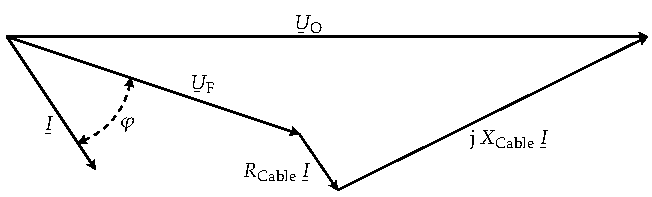
\includegraphics{Imatges/Cap-Cables-Caiguda-Tensio.pdf}
   \caption{Caiguda de tensi\'{o} en corrent altern}\label{pic:cdt_ca}
\end{figure}

Quan es tracta de corrent monof\`{a}sic, la resist\`{e}ncia del cable es calcula segons l'equaci\'{o}
\eqref{eq:r_cc_mono}; la react\`{a}ncia del cable $X\ped{Cable}$ es calcula de forma an\`{a}loga
amb la mateixa equaci\'{o}, a partir de la react\`{a}ncia dels conductors $X\ped{Conductor}$.

Pel que fa al corrent trif\`{a}sic, se suposa equilibrat, i per tant s'utilitza l'equaci\'{o}
\eqref{eq:r_trifas} per calcular la resist\`{e}ncia del cable $R\ped{Cable}$ (i de forma
an\`{a}loga la react\`{a}ncia $X\ped{Cable}$). Addicionalment, els corrents fan refer\`{e}ncia als
corrents de fase, i les tensions a les tensions fase--neutre; l'angle $\varphi$ \'{e}s per
tant l'angle entre la tensi\'{o} final fase--neutre i el corrent de fase.

Disposem en aquest cas de dues equacions, una d'exacta i una altre d'aproximada (per a valors elevats de $\cos \varphi$) .
\begin{subequations}
\begin{align}
   \Delta U &= |\cmplx{I}| ( R\ped{Cable} \cos \varphi + X\ped{Cable} \sin \varphi) + |\cmplx{U}\ped{O}| - \sqrt{|\cmplx{U}\ped{O}|^2 - |\cmplx{I}|^2 ( X\ped{Cable} \cos \varphi - R\ped{Cable} \sin \varphi )^2} \label{eq:cdt_trif_exact} \\
   \Delta U &\approx |\cmplx{I}| ( R\ped{Cable} \cos \varphi + X\ped{Cable} \sin \varphi) \qquad \text{si} \; \cos \varphi \gtrapprox 0{,}8 \label{eq:cdt_trif_aprox}
\end{align}
\end{subequations}

\begin{exemple}
   Es tracta de calcular la caiguda de tensi\'{o} d'un cable, en un sistema trif\`{a}sic on $|\cmplx{U}\ped{O}| = 380\unit{V}$ (fase--fase), $|\cmplx{I}|=630\unit{A}$ i $\cos \varphi = 0{,}87$(i); cada fase est\`{a} formada per tres conductors unipolars de $240\unit{mm^2}$ de secci\'{o} i $400\unit{m}$ de llargada, amb uns valors de resist\`{e}ncia i induct\`{a}ncia de $0{,}095\unit{\ohm/km}$ i $0{,}102\unit{\ohm/km}$ respectivament.

A partir de l'equaci\'{o} \eqref{eq:r_trifas} calculem els valors de $R\ped{Cable}$ i de $X\ped{Cable}$.
\[
   R\ped{Cable} = \frac{0{,}095\unit{\ohm/km}\cdot 0{,}4\unit{km}}{3} = 0{,}0127\unit{\ohm}
\]
\[
   X\ped{Cable} = \frac{0{,}102\unit{\ohm/km}\cdot 0{,}4\unit{km}}{3} = 0{,}0136\unit{\ohm}
\]

Obtenim a continuaci\'{o} el valor de $\sin \varphi$:
\[
   \sin \varphi = \sqrt{1-0{,}87^2} = 0,49
\]

Calculem en primer lloc la caiguda de tensi\'{o} de forma aproximada utilitzant l'equaci\'{o} \eqref{eq:cdt_trif_aprox}.
\[
   \Delta U \approx 630\unit{A} \cdot ( 0{,}0127\unit{\ohm} \cdot 0{,}87 + 0{,}0136\unit{\ohm} \cdot 0{,}49 ) = 11{,}16\unit{V}
\]

que en tant per cent respecte la tensi\'{o} a l'origen representa:
$\frac{11{,}16\unit{V}}{380/\sqrt{3}\unit{V}} \cdot 100 = 5{,}09\unit{\%} $

Finalment, calculem la caiguda de tensi\'{o} exacta utilitzant l'equaci\'{o} \eqref{eq:cdt_trif_exact}.
\[ \begin{split}
   \Delta U &=  630\unit{A} \cdot ( 0{,}0127\unit{\ohm} \cdot 0{,}87 + 0{,}0136\unit{\ohm} \cdot 0{,}49 ) + \frac{380}{\sqrt{3}}\unit{V} \,- \\
    & \quad - \sqrt{(380/\sqrt{3}\unit{V})^2 - (630\unit{A})^2 \cdot ( 0{,}0136\unit{\ohm} \cdot 0{,}87 - 0{,}0127\unit{\ohm} \cdot 0{,}49 )^2 } \,= 11{,}19\unit{V}
\end{split} \]

que en tant per cent respecte la tensi\'{o} a l'origen representa:
$\frac{11{,}19\unit{V}}{380/\sqrt{3}\unit{V}} \cdot 100 = 5{,}10\unit{\%} $
\end{exemple}

\section{Capacitat t\`{e}rmica en curt circuit}\index{cables!capacitat t\`{e}rmica en curt circuit}

Quan hi ha un curt circuit en un cable, tot el calor generat no es transmet a l'exterior, sin\'{o} que s'acumula en la massa del conductor, incrementant la seva temperatura (proc\'{e}s adiab\`{a}tic). En aquestes condicions es pot aplicar l'equaci\'{o}:
\begin{equation}\label{eq:Icc_termica}
   I\ped{cc} = S\, \frac{\text{C}}{\sqrt{t}} \quad
   \begin{cases}
   I\ped{cc} &:\; \text{expressat en\unit{A}} \\
   S         &:\; \text{expressat en\unit{mm^2}} \\
   t         &:\; \text{expressat en\unit{s}} \\
   \text{C}  &:\; \text{par\`{a}metre dependent del tipus de cable}
   \end{cases}
\end{equation}

$I\ped{cc}$ \'{e}s la intensitat de curt circuit que circula pel conductor, $S$ \'{e}s la secci\'{o} del conductor, $t$ \'{e}s el temps m\`{a}xim que pot durar el curt circuit sense que es malmeti el cable, i C \'{e}s un par\`{a}metre que dep\`{e}n del material  del conductor i del seu a\"{\i}llament. En la Taula \vref{taula:const_termica} es donen valors\footnote{Valors obtinguts del cat\`{a}leg del fabricant {"<}General Cable{">}.} de C per a diferents materials del conductor i de l'a\"{\i}llament.
\begin{table}[htb]
   \caption{\label{taula:const_termica} Valors de C pel c\`{a}lcul de curt circuits en cables}
   \begin{center}\begin{tabular}{c>{\hspace{2.5em}}cc}
   \toprule[1pt]
   \renewcommand*{\multirowsetup}{\centering}
   \multirow{2}{25mm}{\rule{0mm}{4mm}Material del\\conductor} & \multicolumn{2}{c}{C, segons el material de l'a\"{\i}llament} \\ \cmidrule(rl){2-3}
    & PVC & EPR i XLPE \\
   \midrule
   Cu & 115 & 142 \\
   Al & 75 & 93 \\
   \bottomrule[1pt]
   \end{tabular} \end{center}
\end{table}
\begin{exemple}
   Es tracta de calcular el temps m\`{a}xim durant el qual un cable de coure de $50\unit{mm^2}$ amb a\"{\i}llament d'EPR, pot suportar un corrent de curt circuit de $15\unit{kA}$.

A partir de l'equaci\'{o} \eqref{eq:Icc_termica} calculem el temps m\`{a}xim demanat:
\[
   t = \left( \frac{S\,C}{I\ped{cc}} \right) ^2 = \left( \frac{50\unit{mm^2}\cdot 142}{15000\unit{A}} \right) ^2 = 0{,}224\unit{s}
\]
\end{exemple}

\section{Conversi\'{o} entre unitats americanes i unitats SI}

\subsection{{"<}Mils{">} (mil), {"<}circular mils{">} (cmil o CM) i {"<}thousand circular mils{">} (kcmil o MCM)}\label{sec:MCM}
\index{mil}\index{cmil}\index{CM}\index{kcmil}\index{MCM}
\index{mils@\guillemotleft mils\guillemotright} \index{circular mils@\guillemotleft circular mils\guillemotright} \index{thousand circular mils@\guillemotleft thousand circular mils\guillemotright}

\index{mils@\guillemotleft mils\guillemotright!difinici\'{o}} \index{circular mils@\guillemotleft circular mils\guillemotright!difinici\'{o}} \index{thousand circular mils@\guillemotleft thousand circular mils\guillemotright!difinici\'{o}}Les definicions d'aquestes tres unitats utilitzades en la mesura de di\`{a}metres i seccions de cables s\'{o}n:
\begin{align}
  1\unit{mil} &\equiv \text{Una mi{\l.l}\`{e}sima de polsada} \\
  1\unit{cmil} = 1\unit{CM} &\equiv  \text{\`{A}rea d'un cercle de di\`{a}metre igual a 1\unit{mil}} \\
  1\unit{kcmil} = 1\unit{MCM} &\equiv 1000\unit{cmil} = 1000\unit{CM}
\end{align}

\index{mils@\guillemotleft mils\guillemotright!equival\`{e}ncies} \index{circular mils@\guillemotleft circular mils\guillemotright!equival\`{e}ncies} \index{thousand circular mils@\guillemotleft thousand circular mils\guillemotright!equival\`{e}ncies}Es donen a continuaci\'{o} algunes conversions d'aquestes unitats:
\begin{align}
   1\unit{mil} &= 10^{-3}\unit{in}  \\
  1\unit{mil} &= 10^{-3}\unit{in} \cdot \frac{25{,}4\unit{mm}}{1\unit{in}} = 25{,}4 \cdot 10^{-3}\unit{mm}  \\
  1\unit{cmil} &= \frac{\piup}{4}\unit{mil^2} = 0{,}785398\unit{mil^2}   \\
   1\unit{cmil} &= \frac{\piup}{4}\cdot 10^{-6}\unit{in^2} = 0{,}785398\cdot 10^{-6}\unit{in^2} \\
   1\unit{cmil} &= \frac{\piup}{4} \cdot 10^{-6}\unit{in^2} \cdot \frac{645{,}16\unit{mm^2}}{1\unit{in^2}} = 506{,}7075\cdot 10^{-6}\unit{mm^2}
   \\[1ex]
   1\unit{kcmil} &= 785{,}398\unit{mil^2}  = 0{,}785398\cdot 10^{-3}\unit{in^2} = 0{,}5067075\unit{mm^2}
\end{align}

Una relaci\'{o} \'{u}til entre di\`{a}metres  i seccions, \'{e}s la seg\"{u}ent: la secci\'{o} $S$ d'un cercle expressada en {"<}circular mils{">}, es igual al quadrat del di\`{a}metre $d$ del cercle expressat en {"<}mils{">}.
\begin{equation}
   S = d^2 \quad
   \begin{cases}
   S &:\; \text{expressat en\unit{cmil}} \\
   d &:\; \text{expressat en\unit{mil}}
   \end{cases}
\end{equation}

En la Taula \vref{taula:MCM} es relacionen els di\`{a}metres i seccions en diverses unitats, dels conductors usualment disponibles compresos entre $2000\unit{kcmil}$ i $250\unit{kcmil}$.
\begin{longtable}{r<{\hspace{0.6em}}rrrrr}
\caption{\label{taula:MCM}Dimensions de cables definits en kcmil} \\
\toprule[1pt]
    \multicolumn{3}{c}{Secci\'{o}} &   \multicolumn{3}{c}{Di\`{a}metre}         \\
    \cmidrule(rl){1-3} \cmidrule(rl){4-6}
    \multicolumn{1}{c}{[kcmil]}  &    \multicolumn{1}{c}{[\unit{in^2}]}  & \multicolumn{1}{c}{[\unit{mm^2}]}  & \multicolumn{1}{c}{[mil]}
           &    \multicolumn{1}{c}{[in]} &   \multicolumn{1}{c}{[mm]}   \\
\midrule \endfirsthead
\caption[]{(\emph{ve de la p\`{a}gina anterior})} \\
\toprule[1pt]
    \multicolumn{3}{c}{Secci\'{o}} &   \multicolumn{3}{c}{Di\`{a}metre}         \\
    \cmidrule(rl){1-3} \cmidrule(rl){4-6}
    \multicolumn{1}{c}{[kcmil]}  &    \multicolumn{1}{c}{[\unit{in^2}]}  & \multicolumn{1}{c}{[\unit{mm^2}]}  & \multicolumn{1}{c}{[mil]}
           &    \multicolumn{1}{c}{[in]} &   \multicolumn{1}{c}{[mm]}   \\
\midrule \endhead
\midrule
\multicolumn{6}{r}{(\emph{continua a la p\`{a}gina seg\"{u}ent})}
\endfoot
\endlastfoot
2000 &   1,570796 &  1013,4150 & 1414,21356 &  1,4142136 &   35,92102 \\
1750 &   1,374447 &   886,7381 & 1322,87566 &  1,3228757 &   33,60104 \\
1600 &   1,256637 &   810,7320 & 1264,91106 &  1,2649111 &   32,12874 \\
1500 &   1,178097 &   760,0612 & 1224,74487 &  1,2247449 &   31,10852 \\
1250 &   0,981748 &   633,3843 & 1118,03399 &  1,1180340 &   28,39806 \\
1000 &   0,785398 &   506,7075 & 1000,00000 &  1,0000000 &   25,40000 \\
 800 &   0,628319 &   405,3660 &  894,42719 &  0,8944272 &   22,71845 \\
 750 &   0,589049 &   380,0306 &  866,02540 &  0,8660254 &   21,99705 \\
 700 &   0,549779 &   354,6952 &  836,66003 &  0,8366600 &   21,25116 \\
 600 &   0,471239 &   304,0245 &  774,59667 &  0,7745967 &   19,67476 \\
 500 &   0,392699 &   253,3537 &  707,10678 &  0,7071068 &   17,96051 \\
 450 &   0,353429 &   228,0184 &  670,82039 &  0,6708204 &   17,03884 \\
 400 &   0,314159 &   202,6830 &  632,45553 &  0,6324555 &   16,06437 \\
 350 &   0,274889 &   177,3476 &  591,60798 &  0,5916080 &   15,02684 \\
 300 &   0,235619 &   152,0122 &  547,72256 &  0,5477226 &   13,91215 \\
 250 &   0,196350 &   126,6769 &  500,00000 &  0,5000000 &   12,70000 \\
\bottomrule[1pt]
\end{longtable}

D'aquesta taula es pot veure que: $\text{Secci\'{o} en}\unit{mm^2} \approx \dfrac{\text{Secci\'{o} en}\unit{kcmil}}{2}$.

\break
\subsection{{"<}American Wire Gauge{">} (AWG)}
\index{AWG (\guillemotleft American Wire Gauge\guillemotright)}

\index{AWG (\guillemotleft American Wire Gauge\guillemotright)!definici\'{o}}L'{"<}American Wire Gauge{">}, anomenat tamb\'{e} {"<}Brown \& Sharp Gauge{">}, \'{e}s un sistema de numeraci\'{o} de conductors de coure segons el seu di\`{a}metre. A cada n\'{u}mero AWG correspon un valor de di\`{a}metre; els successius di\`{a}metres formen una progressi\'{o} geom\`{e}trica descendent (en augmentar el n\'{u}mero AWG, disminueix el di\`{a}metre).

La ra\'{o} d'aquesta progressi\'{o} geom\`{e}trica s'obt\'{e} de la seg\"{u}ent consideraci\'{o}: hi ha dos valors de refer\`{e}ncia, AWG 36, al qual s'assigna un di\`{a}metre de 5\unit{mil}, i AWG 4/0 (tamb\'{e} anomenat AWG 0000), al qual s'assigna un di\`{a}metre de 460\unit{mil}. Entre aquest dos valors de refer\`{e}ncia hi ha una diferencia de 39 unitats (vegeu la Taula \vref{taula:AWG}), i per tant, sent $r\ped{d}$ la ra\'{o} de di\`{a}metres buscada, tenim:
\begin{equation}
   5\unit{mil} = 460\unit{mil} \cdot r\ped{d}^{39} \quad \rightarrow \quad r\ped{d} = \left( \frac{5\unit{mil}}{460\unit{mil}} \right)^{1/39} = \left( \frac{1}{92} \right)^{1/39} = 92^{-1/39}
\end{equation}

En ser la secci\'{o} d'un conductor proporcional al quadrat del seu di\`{a}metre, les seccions dels successius n\'{u}meros AWG formen una progressi\'{o} geom\`{e}trica  descendent de ra\'{o} $r\ped{S}$ igual a: \begin{equation}
   r\ped{S} = r\ped{d}^2 = 92^{-2/39}
\end{equation}

Finalment, en ser la resist\`{e}ncia d'un conductor inversament proporcional a la seva secci\'{o}, les resist\`{e}ncies dels successius n\'{u}meros AWG formen una progressi\'{o} geom\`{e}trica ascendent de ra\'{o} $r\ped{R}$ igual a:
\begin{equation}
   r\ped{R} = \frac{1}{r\ped{S}} = 92^{2/39}
\end{equation}

A partir d'aquestes raons, i coneixent el di\`{a}metre $d$, la secci\'{o} $S$ i la resist\`{e}ncia $R$ d'un n\'{u}mero AWG $n$, podem calcular aquests par\`{a}metres per a un altre n\'{u}mero AWG, $k$ unitats posterior o $k$ unitats anterior:

\begin{equation}
   \begin{array}{rllllll}
     \text{AWG:}         & & n & & n+k                & & n-k \\
     \text{Di\`{a}metre:}    & & d & & d\cdot 92^{-k/39}  & & d\cdot 92^{k/39} \\
     \text{Secci\'{o}:}      & & S & & S\cdot 92^{-2k/39} & & S\cdot 92^{2k/39} \\
     \text{Resist\`{e}ncia:} & & R & & R\cdot 92^{2k/39}  & & R\cdot 92^{-2k/39}
   \end{array}
\end{equation}

Per a alguns valors particulars de $k$, es compleixen de forma aproximada les seg\"{u}ents relacions:

\begin{list}{}
   {\setlength{\labelwidth}{15mm} \setlength{\leftmargin}{17mm} \setlength{\labelsep}{2mm}}

   \item[$k=6$\hfill] En augmentar en 6  unitats el n\'{u}mero AWG, el di\`{a}metre es divideix per 2
                 $(92^{-6/39}\approx 0{,}5)$.

   \item[$k=-6$\hfill] En disminuir en 6 unitats el n\'{u}mero AWG, el di\`{a}metre es multiplica per 2
                 $(92^{6/39}\approx 2)$.

   \item[$k=20$\hfill] En augmentar en 20  unitats el n\'{u}mero AWG, el di\`{a}metre es divideix per 10
                 $(92^{-20/39}\approx 0{,}1)$.

   \item[$k=-20$\hfill] En disminuir en 20 unitats el n\'{u}mero AWG, el di\`{a}metre es multiplica per 10
                 $(92^{20/39}\approx 10)$.

   \item[$k=3$\hfill] En augmentar en 3 unitats el n\'{u}mero AWG, la secci\'{o} es divideix per 2
                 $(92^{-2\cdot3/39}\approx 0{,}5)$ i la resist\`{e}ncia es multiplica per 2
                 $(92^{2\cdot3/39}\approx 2)$.

   \item[$k=-3$\hfill] En disminuir en 3 unitats el n\'{u}mero AWG, la secci\'{o} es multiplica per 2
                  $(92^{2\cdot3/39}\approx 2)$ i la resist\`{e}ncia es divideix per 2
                  $(92^{-2\cdot3/39}\approx 0{,}5)$.

   \item[$k=10$\hfill] En augmentar en 10 unitats el n\'{u}mero AWG, la secci\'{o} es divideix per 10
                 $(92^{-2\cdot10/39}\approx 0{,}1)$ i la resist\`{e}ncia es multiplica per 10
                 $(92^{2\cdot10/39}\approx 10)$.

   \item[$k=-10$\hfill] En disminuir en 10 unitats el n\'{u}mero AWG, la secci\'{o} es multiplica per 10
                  $(92^{2\cdot10/39}\approx 10)$ i la resist\`{e}ncia es divideix per 10
                  $(92^{-2\cdot10/39}\approx 0{,}1)$.
\end{list}

\index{AWG (\guillemotleft American Wire Gauge\guillemotright)!equival\`{e}ncies}En la Taula \vref{taula:AWG} es relacionen els di\`{a}metres i seccions en diverses unitats dels conductors compresos entre AWG 4/0 i AWG 50.



\begin{longtable}{crrrrrr}
\caption{\label{taula:AWG}Dimensions de cables AWG} \\
\toprule[1pt]
    \renewcommand*{\multirowsetup}{\centering}
    \multirow{2}{12mm}{\rule{0mm}{4mm}Cable\\{[AWG]}}  &    \multicolumn{3}{c}{Di\`{a}metre} &   \multicolumn{3}{c}{Secci\'{o}}         \\
    \cmidrule(rl){2-4} \cmidrule(rl){5-7}
      &    \multicolumn{1}{c}{[mil]}  & \multicolumn{1}{c}{[in]}  & \multicolumn{1}{c}{[mm]}
           &    \multicolumn{1}{c}{[cmil]} &   \multicolumn{1}{c}{[\unit{in^2}]}  & \multicolumn{1}{c}{[\unit{mm^2}]} \\
\midrule \endfirsthead
\caption[]{Dimensions de cables AWG (\emph{ve de la p\`{a}gina anterior})} \\
\toprule[1pt]
    \renewcommand*{\multirowsetup}{\centering}
    \multirow{2}{12mm}{\rule{0mm}{4mm}Cable\\{[AWG]}}  &    \multicolumn{3}{c}{Di\`{a}metre} &   \multicolumn{3}{c}{Secci\'{o}}         \\
    \cmidrule(rl){2-4} \cmidrule(rl){5-7}
      &    \multicolumn{1}{c}{[mil]}  & \multicolumn{1}{c}{[in]}  & \multicolumn{1}{c}{[mm]}
           &    \multicolumn{1}{c}{[cmil]} &   \multicolumn{1}{c}{[\unit{in^2}]}  & \multicolumn{1}{c}{[\unit{mm^2}]} \\
\midrule \endhead
\midrule
\multicolumn{7}{r}{(\emph{continua a la p\`{a}gina seg\"{u}ent})}
\endfoot
\endlastfoot


 4/0  &    460,000 &   0,460000 &    11,6840 & 211600,000 &  1,662$\cdot 10^{-1}$ & 107,219303 \\
 3/0  &    409,642 &   0,409642 &    10,4049 & 167806,429 &  1,318$\cdot 10^{-1}$ &  85,028773 \\
 2/0  &    364,797 &   0,364797 &     9,2658 & 133076,548 &  1,045$\cdot 10^{-1}$ &  67,430882 \\
 1/0  &    324,861 &   0,324861 &     8,2515 & 105534,501 &  8,289$\cdot 10^{-2}$ &  53,475121 \\
 1 &    289,297 &   0,289297 &     7,3481 &  83692,664 &  6,573$\cdot 10^{-2}$ &  42,407699 \\
 2 &    257,626 &   0,257626 &     6,5437 &  66371,300 &  5,213$\cdot 10^{-2}$ &  33,630834 \\
 3 &    229,423 &   0,229423 &     5,8273 &  52634,834 &  4,134$\cdot 10^{-2}$ &  26,670464 \\
 4 &    204,307 &   0,204307 &     5,1894 &  41741,321 &  3,278$\cdot 10^{-2}$ &  21,150639 \\
 5 &    181,941 &   0,181941 &     4,6213 &  33102,372 &  2,600$\cdot 10^{-2}$ &  16,773220 \\
 6 &    162,023 &   0,162023 &     4,1154 &  26251,375 &  2,062$\cdot 10^{-2}$ &  13,301768 \\
 7 &    144,285 &   0,144285 &     3,6649 &  20818,287 &  1,635$\cdot 10^{-2}$ &  10,548782 \\
 8 &    128,490 &   0,128490 &     3,2636 &  16509,652 &  1,297$\cdot 10^{-2}$ &   8,365564 \\
 9 &    114,424 &   0,114424 &     2,9064 &  13092,749 &  1,028$\cdot 10^{-2}$ &   6,634194 \\
10 &    101,897 &   0,101897 &     2,5882 &  10383,022 &  8,155$\cdot 10^{-3}$ &   5,261155 \\
11 &     90,742 &   0,090742 &     2,3048 &   8234,111 &  6,467$\cdot 10^{-3}$ &   4,172286 \\
12 &     80,808 &   0,080808 &     2,0525 &   6529,947 &  5,129$\cdot 10^{-3}$ &   3,308773 \\
13 &     71,962 &   0,071962 &     1,8278 &   5178,483 &  4,067$\cdot 10^{-3}$ &   2,623976 \\
14 &     64,084 &   0,064084 &     1,6277 &   4106,724 &  3,225$\cdot 10^{-3}$ &   2,080908 \\
15 &     57,068 &   0,057068 &     1,4495 &   3256,780 &  2,558$\cdot 10^{-3}$ &   1,650235 \\
16 &     50,821 &   0,050821 &     1,2908 &   2582,744 &  2,028$\cdot 10^{-3}$ &   1,308696 \\
17 &     45,257 &   0,045257 &     1,1495 &   2048,209 &  1,609$\cdot 10^{-3}$ &   1,037843 \\
18 &     40,303 &   0,040303 &     1,0237 &   1624,304 &  1,276$\cdot 10^{-3}$ &   0,823047 \\
19 &     35,891 &   0,035891 &     0,9116 &   1288,131 &  1,012$\cdot 10^{-3}$ &   0,652706 \\
20 &     31,961 &   0,031961 &     0,8118 &   1021,535 &  8,023$\cdot 10^{-4}$ &   0,517619 \\
21 &     28,462 &   0,028462 &     0,7229 &    810,114 &  6,363$\cdot 10^{-4}$ &   0,410491 \\
22 &     25,347 &   0,025347 &     0,6438 &    642,449 &  5,046$\cdot 10^{-4}$ &   0,325534 \\
23 &     22,572 &   0,022572 &     0,5733 &    509,486 &  4,001$\cdot 10^{-4}$ &   0,258160 \\
24 &     20,101 &   0,020101 &     0,5106 &    404,040 &  3,173$\cdot 10^{-4}$ &   0,204730 \\
25 &     17,900 &   0,017900 &     0,4547 &    320,419 &  2,517$\cdot 10^{-4}$ &   0,162359 \\
26 &     15,941 &   0,015941 &     0,4049 &    254,104 &  1,996$\cdot 10^{-4}$ &   0,128756 \\
27 &     14,196 &   0,014196 &     0,3606 &    201,513 &  1,583$\cdot 10^{-4}$ &   0,102108 \\
28 &     12,641 &   0,012641 &     0,3211 &    159,807 &  1,255$\cdot 10^{-4}$ &   0,080976 \\
29 &     11,258 &   0,011258 &     0,2859 &    126,733 &  9,954$\cdot 10^{-5}$ &   0,064217 \\
30 &     10,025 &   0,010025 &     0,2546 &    100,504 &  7,894$\cdot 10^{-5}$ &   0,050926 \\
31 &      8,928 &   0,008928 &     0,2268 &     79,703 &  6,260$\cdot 10^{-5}$ &   0,040386 \\
32 &      7,950 &   0,007950 &     0,2019 &     63,207 &  4,964$\cdot 10^{-5}$ &   0,032028 \\
33 &      7,080 &   0,007080 &     0,1798 &     50,126 &  3,937$\cdot 10^{-5}$ &   0,025399 \\
34 &      6,305 &   0,006305 &     0,1601 &     39,752 &  3,122$\cdot 10^{-5}$ &   0,020142 \\
35 &      5,615 &   0,005615 &     0,1426 &     31,524 &  2,476$\cdot 10^{-5}$ &   0,015974 \\
36 &      5,000 &   0,005000 &     0,1270 &     25,000 &  1,963$\cdot 10^{-5}$ &   0,012668 \\
37 &      4,453 &   0,004453 &     0,1131 &     19,826 &  1,557$\cdot 10^{-5}$ &   0,010046 \\
38 &      3,965 &   0,003965 &     0,1007 &     15,723 &  1,235$\cdot 10^{-5}$ &   0,007967 \\
39 &      3,531 &   0,003531 &     0,0897 &     12,469 &  9,793$\cdot 10^{-6}$ &   0,006318 \\
40 &      3,145 &   0,003145 &     0,0799 &      9,888 &  7,766$\cdot 10^{-6}$ &   0,005010 \\
41 &      2,800 &   0,002800 &     0,0711 &      7,842 &  6,159$\cdot 10^{-6}$ &   0,003973 \\
42 &      2,494 &   0,002494 &     0,0633 &      6,219 &  4,884$\cdot 10^{-6}$ &   0,003151 \\
43 &      2,221 &   0,002221 &     0,0564 &      4,932 &  3,873$\cdot 10^{-6}$ &   0,002499 \\
44 &      1,978 &   0,001978 &     0,0502 &      3,911 &  3,072$\cdot 10^{-6}$ &   0,001982 \\
45 &      1,761 &   0,001761 &     0,0447 &      3,102 &  2,436$\cdot 10^{-6}$ &   0,001572 \\
46 &      1,568 &   0,001568 &     0,0398 &      2,460 &  1,932$\cdot 10^{-6}$ &   0,001246 \\
48 &      1,244 &   0,001244 &     0,0316 &      1,547 &  1,215$\cdot 10^{-6}$ &   0,000784 \\
50 &      0,986 &   0,000986 &     0,0251 &      0,973 &  7,641$\cdot 10^{-7}$ &   0,000493 \\
52 &      0,782 &   0,000782 &     0,0199 &      0,612 &  4,805$\cdot 10^{-7}$ &   0,000310
\\
54 &      0,620 &   0,000620 &     0,0158 &      0,385 &  3,022$\cdot 10^{-7}$ &   0,000195
\\
56 &      0,492 &   0,000492 &     0,0125 &      0,242 &  1,901$\cdot 10^{-7}$ &   0,000123
\\
\bottomrule[1pt]
\end{longtable}

\index{AWG (\guillemotleft American Wire Gauge\guillemotright)!conversi\'{o} a\unit{mm^2}} Es d\'{o}na finalment, la f\'{o}rmula per passar directament d'un n\'{u}mero AWG $n$, a la seva secci\'{o} $S$ equivalent expressada en\unit{mm^2}.
\begin{equation}
   S = \frac{25{,}4^2 \cdot 460^2 \cdot \piup}{4 \cdot 10^6 \cdot 92^{2\cdot\frac{n+3}{39}}} =
   53{,}4751207 \cdot 92^{-\frac{n}{19{,}5}} = 53{,}4751207 \cdot \eu^{-n\cdot \frac{\ln 92}{19{,}5} }\label{eq:awg_mm2}
\begin{cases}
   S &:\; \text{expressada en\unit{mm^2}} \\
   n &:\; \text{n\'{u}mero AWG}
\end{cases}
\end{equation}

En aquesta f\'{o}rmula, cal utilitzar els valors $n = 0$, -1, -2, i -3,  pels n\'{u}meros AWG 1/0,
2/0, 3/0 i 4/0 respectivament.
